\documentclass[aspectratio=169]{beamer}
\usepackage[utf8]{inputenc}
\usepackage[T1]{fontenc}

\usepackage{theme/beamerthemeNBersp}


\title{Modulación de fase en ondas de Faraday}
\subtitle{Charla de avance de Laboratorio 7}
\author{
	Bernardo Español \and Melisa Vinograd
	\texorpdfstring{\\ \vspace{0.1cm} Dirección: Dr. Pablo Cobelli}{}
}
\institute{Laboratorio de Turbulencia Geofísica, FLiP: Fluidos y Plasmas}
\date{} 

\begin{document}

% Título
\begin{frame}[noframenumbering,plain]
	\titlepage
\end{frame}

\section{Recapitulación}

\begin{frame}{Montaje experimental}
	\begin{figure}[ht]
		\centering
		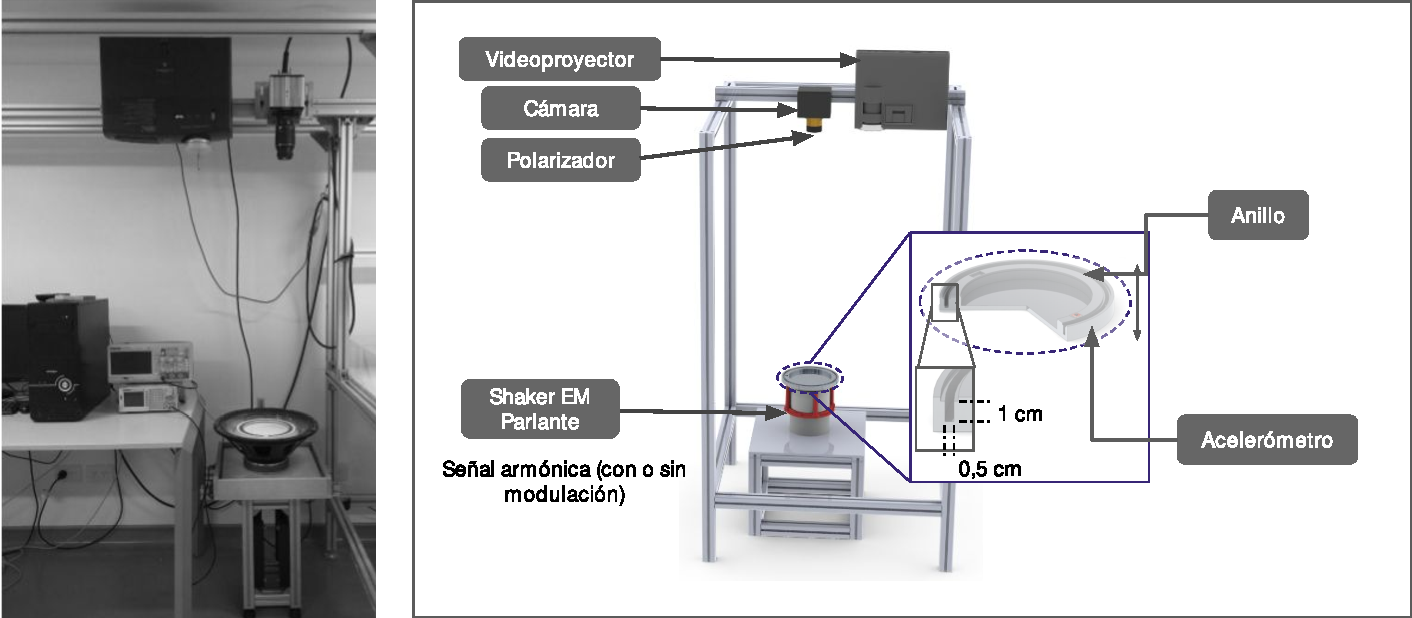
\includegraphics[width=1\textwidth]{figs/esquema_experimental.pdf}
	\end{figure}
\end{frame}

\begin{frame}{Extracción de la superficie libre}
	\begin{minipage}{0.49\textwidth}
	  \begin{figure}
	    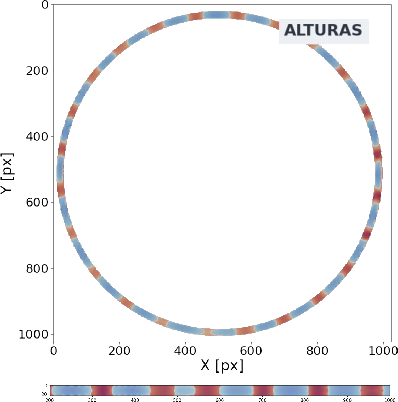
\includegraphics[width=0.8\linewidth]{figs/anillo_a_strip.png}
	  \end{figure}
	\end{minipage} \hfill
	\begin{minipage}{0.49\textwidth}
	  \begin{figure}
	    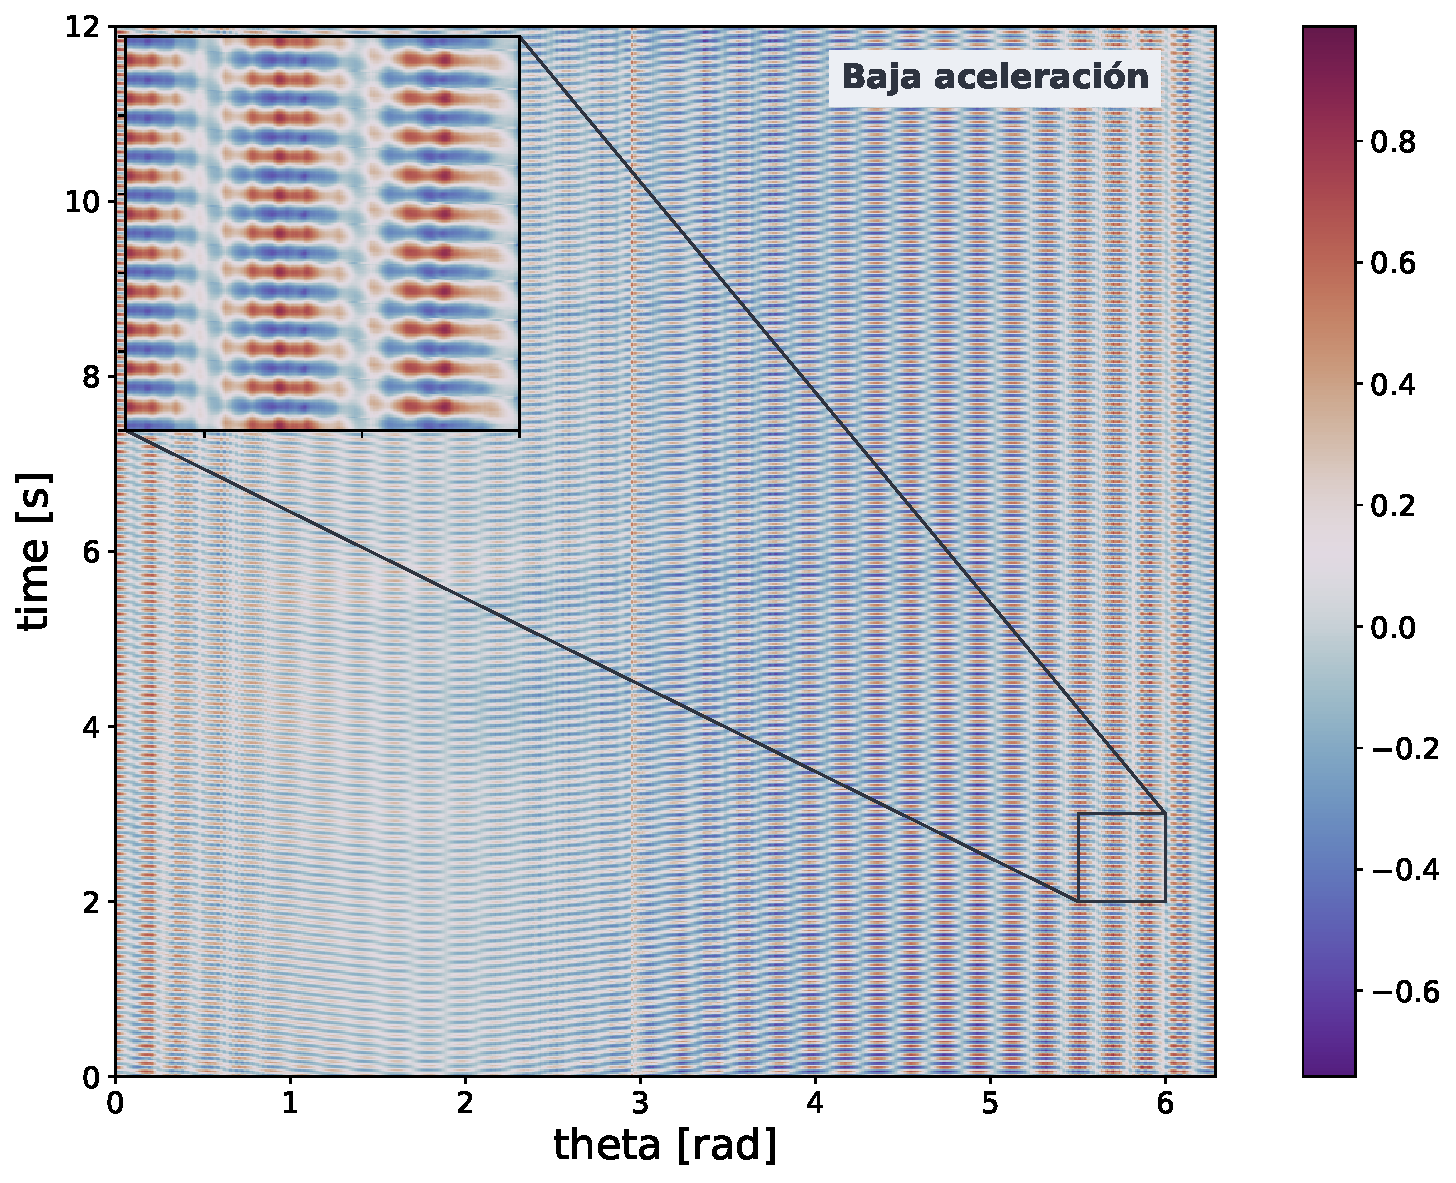
\includegraphics[width=\linewidth]{figs/st_MED5.pdf}
	  \end{figure}
	\end{minipage}
	% TODO[meli]: Volver a exportar
\end{frame}

\section{Avances}

\begin{frame}{Avances en el código}
	\begin{itemize} 
		\item Paralelización
			\vspace{0.8cm}
		\item Transformación de fase a alturas
			\vspace{0.8cm}
		\item Unwrapping temporal
			\vspace{0.8cm}
		\item Herramientas de visualización
	\end{itemize}
\end{frame}

\begin{frame}{Corrección de errores en los diagramas espacio-temporales}
	\begin{figure}[ht]
		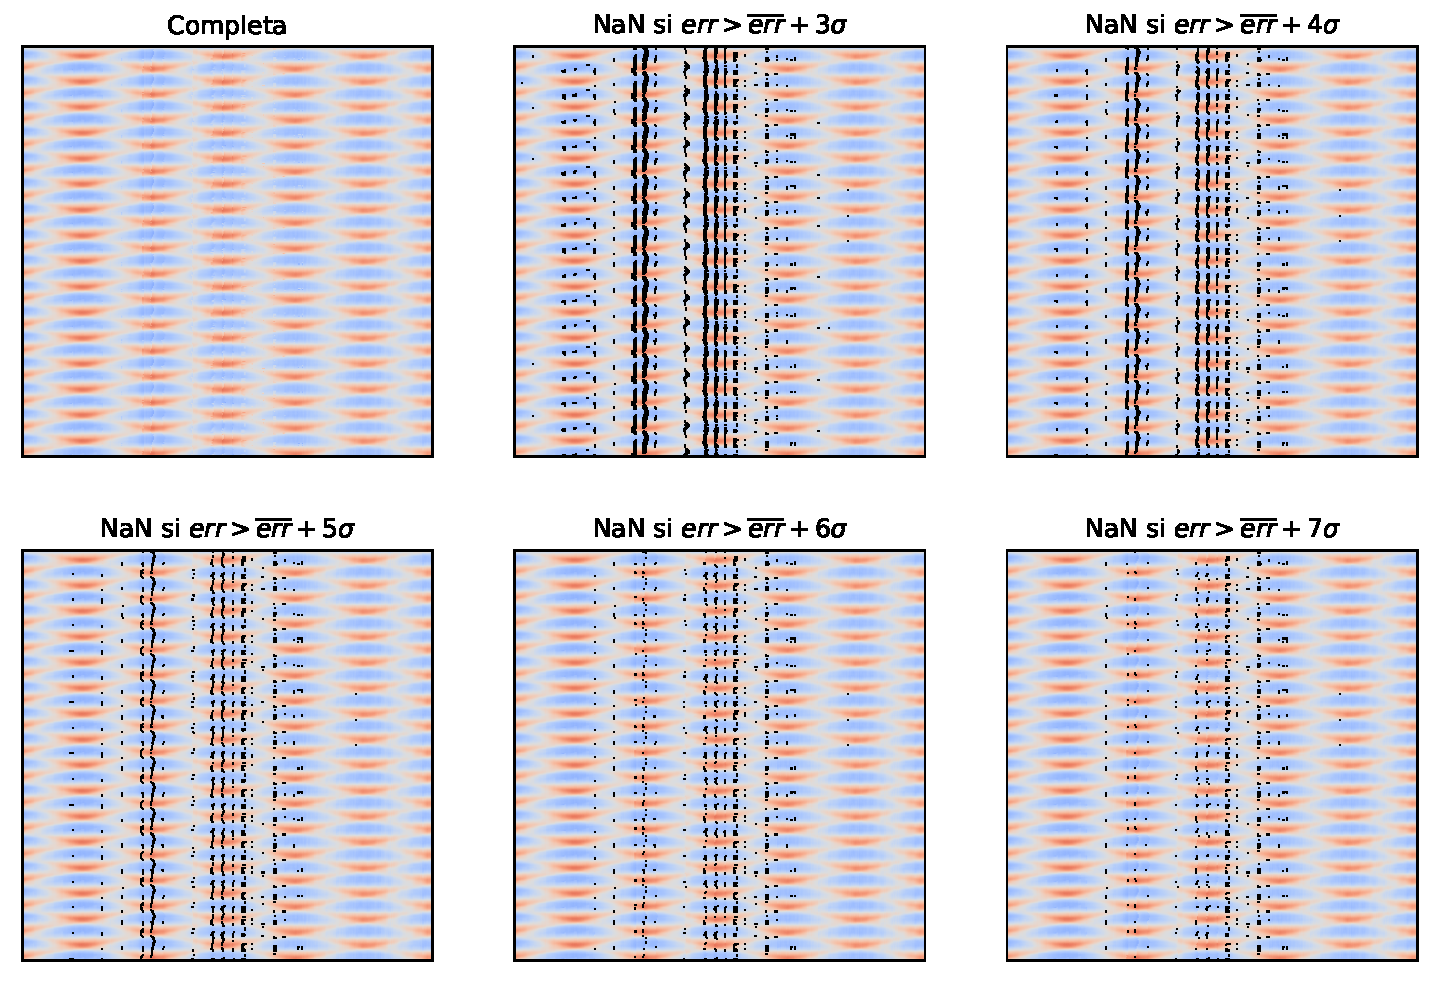
\includegraphics[width=0.75\linewidth]{figs/error_analysis.pdf}
	\end{figure}
\end{frame}
\begin{frame}{Corrección de errores en los diagramas espacio-temporales}
	\begin{figure}[ht]
		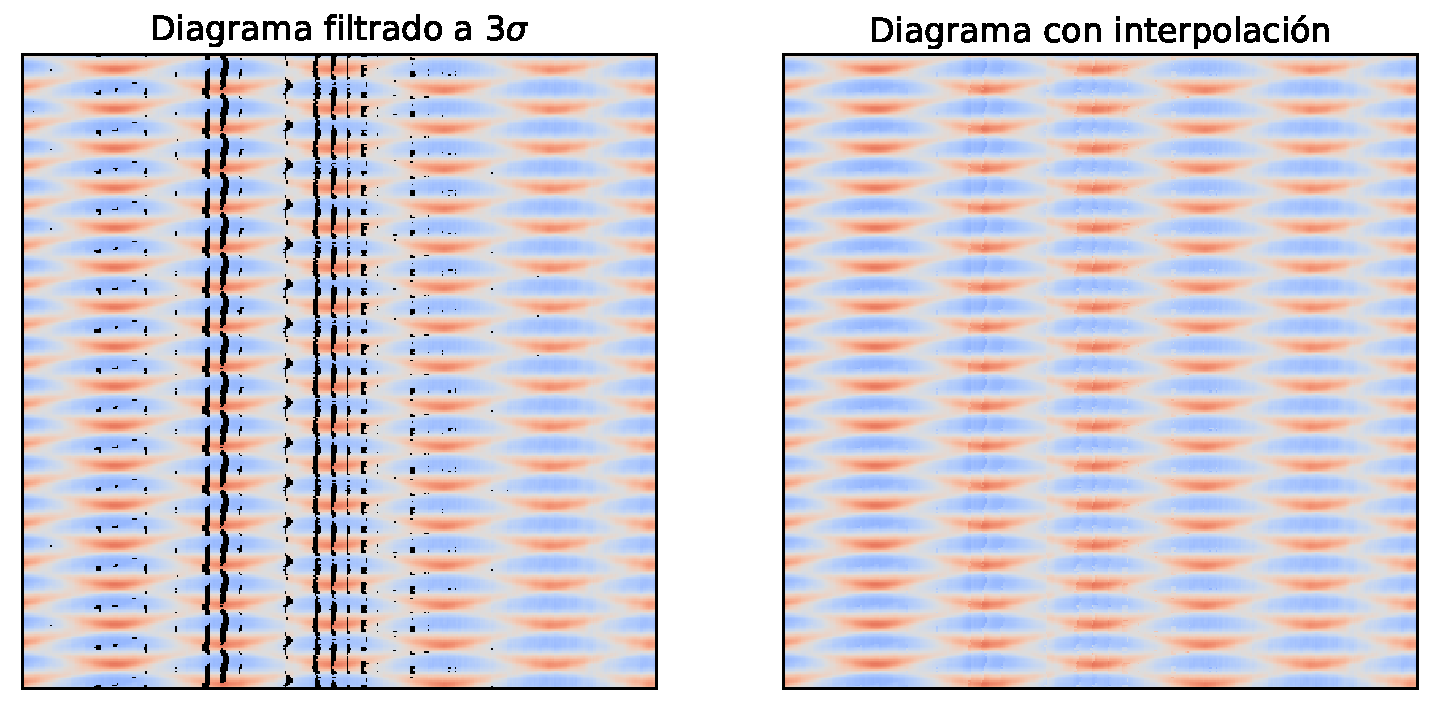
\includegraphics[width=0.8\linewidth]{figs/error_interp.pdf}
	\end{figure}
	% TODO[berna]: Exportar con 3 sigmas
\end{frame}

\begin{frame}{Envolvente de la superficie libre}
	\begin{figure}[ht]
		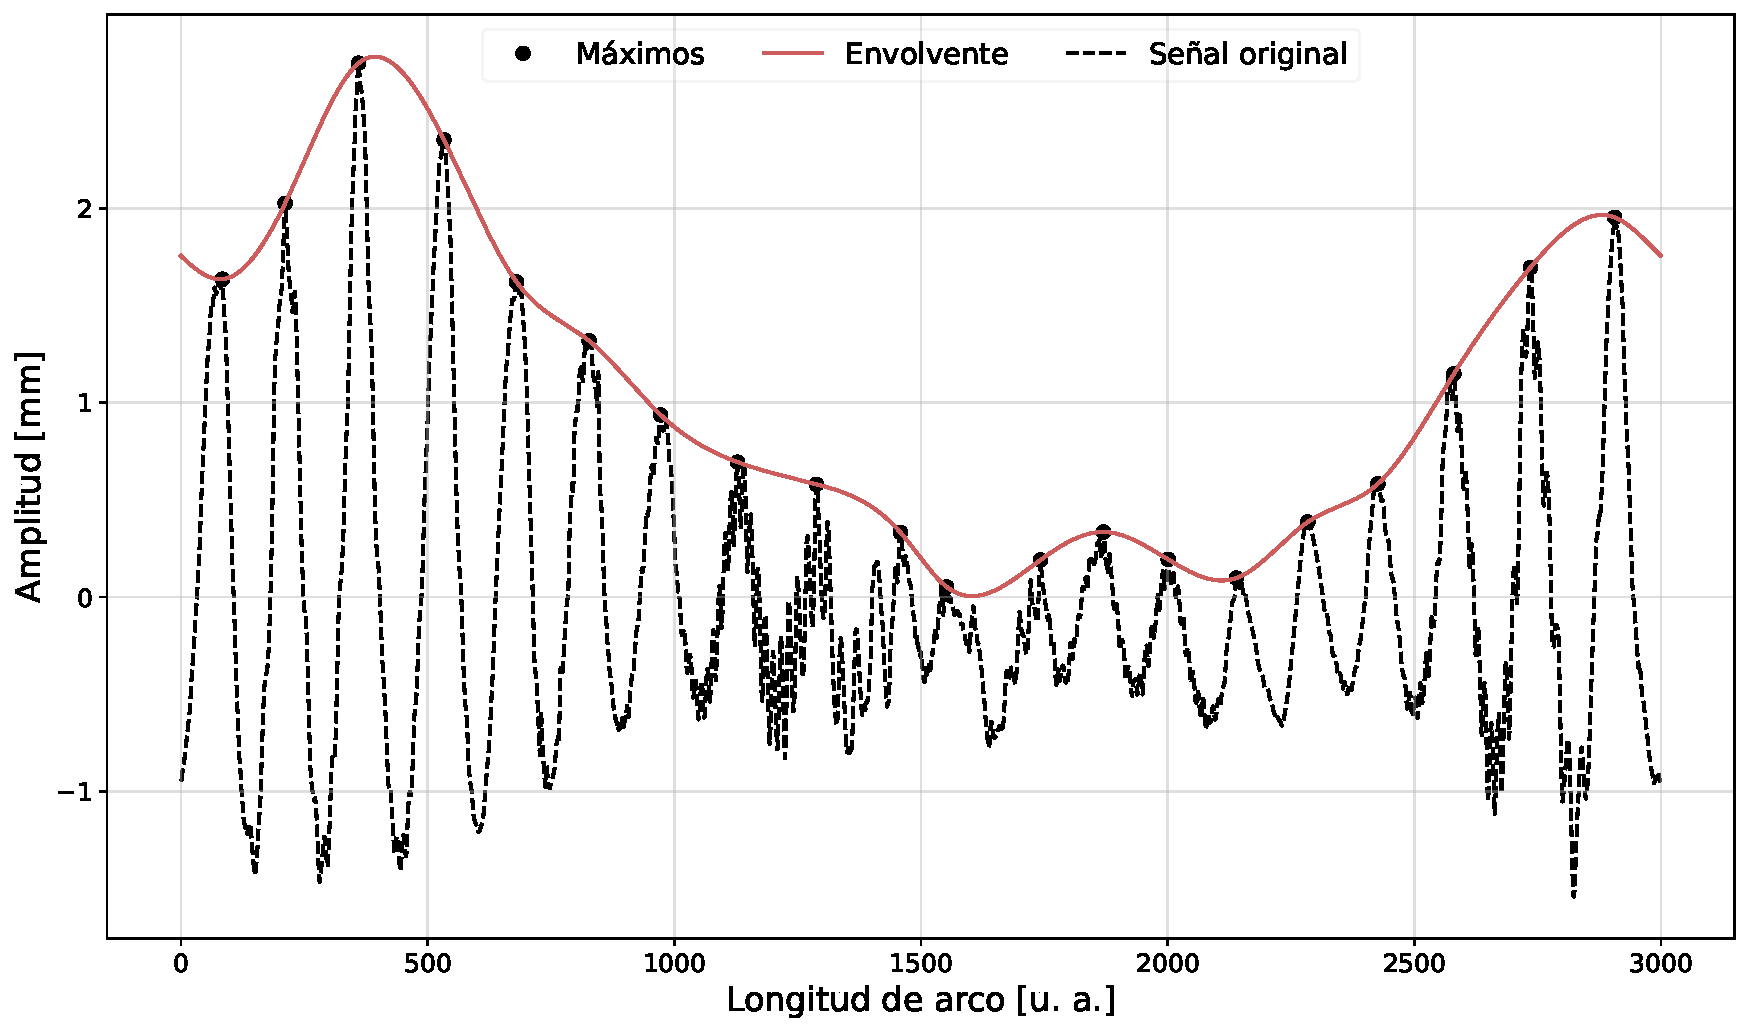
\includegraphics[width=0.9\textwidth]{figs/env_1sample.pdf}
	\end{figure}
	%TODO[berna]: Sacarle el fondo a la legend
\end{frame}

\begin{frame}{Envolvente de la superficie libre}
	\begin{figure}[ht]
		\centering
		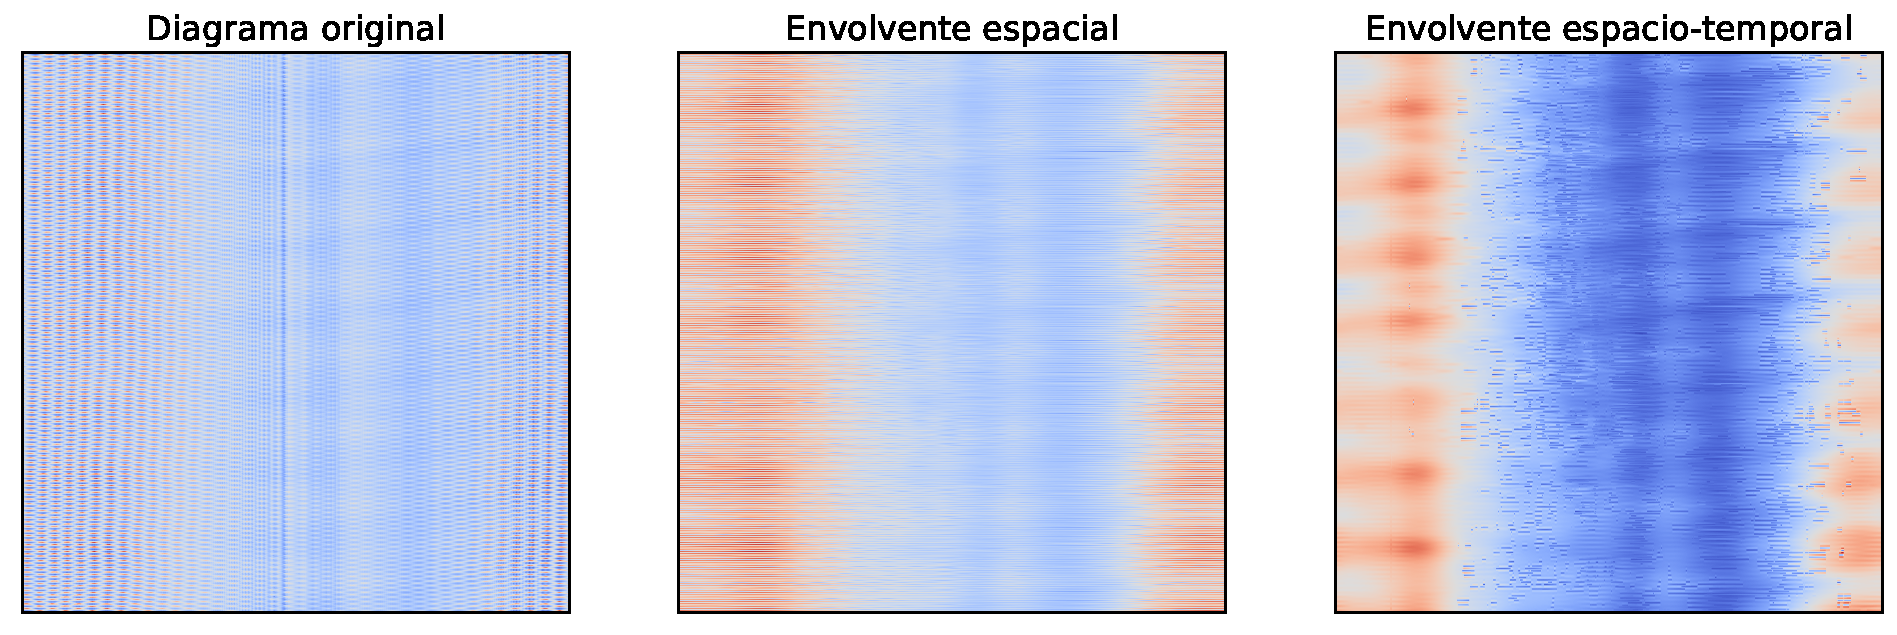
\includegraphics[width=\textwidth]{figs/st_envelopes.pdf}
	\end{figure}
\end{frame}

\begin{frame}{Ondas propagativas}
	\begin{figure}[ht]
		\centering
		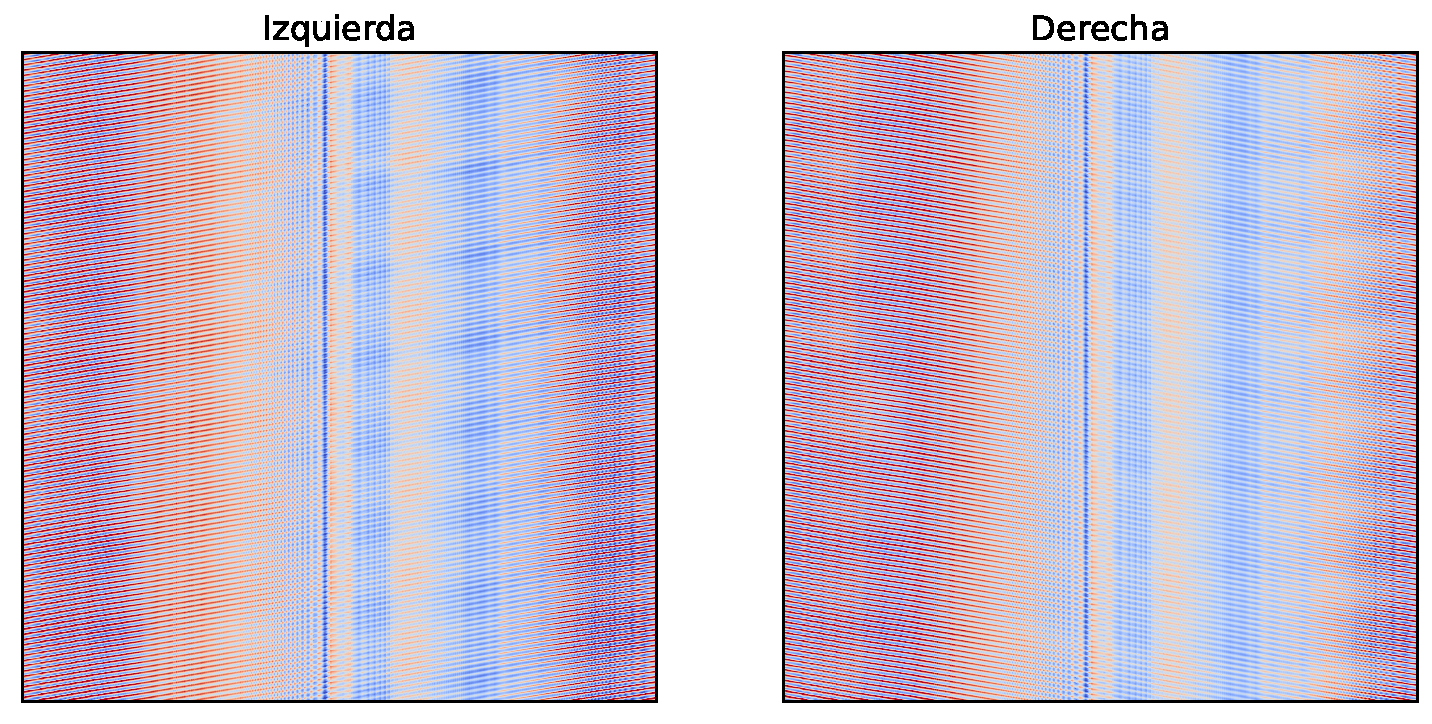
\includegraphics[width=0.8\textwidth]{figs/st_left_right.pdf}
	\end{figure}
\end{frame}

\section{Perspectivas}
\begin{frame}{Mediciones a analizar}
	\begin{itemize} 
		\item Respuesta del sistema aumentando y disminuyendo la aceleración
			\vspace{0.8cm}
		\item Distribución de la energía en los modos del sistema (con y sin modulación)
			\vspace{0.8cm}
		\item Velocidad característica de los trenes de oscilones
			\vspace{0.8cm}
		\item Ajuste de ecuaciones de amplitud
	\end{itemize}
\end{frame}

\section*{Gracias.}

\end{document}
